\chapter{Lagrangian duality}
\label{chap:lagrangian_duality}

Duality is fascinating topic in mathematical optimization: the basic arguments
used in the theory of duality are elementary and yet they can lead to powerful
and far-reaching conclusions.    

\section{LP duality*}
\label{sec:lp_duality}

The story begins, for us, with linear programs (LPs). Consider a generic LP of
the form 
\begin{equation}
\label{eq:lp_primal}
\begin{alignedat}{2}
&\minimize_x \quad && c^\T x \\
&\st \quad && Ax \leq b \\
& && Gx = h, 
\end{alignedat}
\end{equation}
where $c \in \R^d$, $A \in \R^{m \times d}$, $b \in \R^m$, $G \in \R^{k \times 
  d}$, $h \in \R^k$. The reason we start the chapter by studying LPs is that,   
in this problem class, we can build up dual problems ``constructively''; this 
constructive approach is not possible for general optimization problems, and
helps us appreciate the importance and elegance of Lagrange duality, which is
covered next.     

The fundamental question that underlies the study of duality is as follows: what
is the tightest lower bound we can form on the optimal criterion value $f^\star
= c^\T x^\star$ in \eqref{eq:lp_primal}? To address this, suppose that $u \in
\R^m$ and $v \in \R^k$ are arbitrary vectors---which we call \emph{dual 
  variables} in this context---with $u$ nonnegative in each component, $u \geq   
0$. Provided that $x \in \R^d$ is a feasible point for problem
\eqref{eq:lp_primal}, it holds that $u^\T (Ax - b) \leq 0$ and $v^\T (Gx - h) =
0$, and so, adding these together gives        
\begin{equation}
\label{eq:lp_dual_nonnegative}
u^\T (Ax - b) + v^\T (Gx - h) \leq 0.
\end{equation}
In order to obtain a lower bound on the criterion value $c^\T x$, we rearrange
the above into
\[
(-A^\T u - G^\T v)^\T x \geq -b^\T u - h^\T v.
\]
The key observation is that this provides the lower bound we desire provided
that the dual variables $u,v$ are chosen such that $-A^\T u - G^\T v= c$. This
is true for any feasible $x$, thus taking an infimum over all such $x$ gives   
\[
f^\star \geq -b^\T u - h^\T v, \quad \text{for any $u,v$ such that $-A^\T u -
  G^\T v = c$ and $u \geq 0$}.
\]
Finally, to make this lower bound as tight as possible, we maximize the
right-hand side above,  
\begin{equation}
\label{eq:lp_weak_duality}
f^\star \geq \, \underbrace{\sup \big\{ -b^\T u - h^\T v :  A^\T u + G^\T v =
  -c, \, u \geq 0 \big\}}_{g^\star}.
\end{equation}
Now the right-hand side in \eqref{eq:lp_weak_duality}, which we may denote as 
$g^\star = -b^\T u^\star - h^\T v^\star$, is itself the optimal criterion value
associated with an optimization problem, indeed an LP,     
\index{linear program!dual problem}
\begin{equation}
\label{eq:lp_dual}
\begin{alignedat}{2}
&\maximize_{u,v} \quad && -b^\T u - h^\T v \\
&\st \quad && A^\T u + G^\T v = -c \\
& && u \geq 0.
\end{alignedat}
\end{equation}
In this context, we call \eqref{eq:lp_dual} the \emph{dual LP} and the original 
problem \eqref{eq:lp_primal} the \emph{primal LP}. Note that, by construction 
\eqref{eq:lp_weak_duality}, we have $f^\star \geq g^\star$: the optimal value in
the dual problem is a lower bound on the optimal value in the primal problem.   

There are several natural follow-up questions that we can ask: for example, when
does equality hold in \eqref{eq:lp_weak_duality}, $f^\star = g^\star$? And, how 
do solutions $x^\star$ and $u^\star, v^\star$ in \eqref{eq:lp_primal} and
\eqref{eq:lp_dual}, respectively, relate? We will address these questions and
more, over this chapter and the next one. First, however, we must develop a
theory of duality beyond LPs. 

\begin{Remark}
In the attempt to move beyond LPs with the constructive approach to duality, we 
run into a shortcoming: when the criterion $f$ is nonlinear, but the constraint
functions are linear, we have no way in general to combine the
constraints---which are linear equalities and inequalities in $x$---to construct
a lower bound on $f(x)$. But there is another way: Lagrangian duality, as we
will see next, applies seamlessly to LPs and convex optimization more broadly
(and even some nonconvex problems).   
\end{Remark}

\section{Lagrangian duality}
\label{sec:lagrangian_duality}

Lagrangian duality (or Lagrange duality) starts with the same motivation as in
the last section, but cast in a more general setting: we seek a lower bound on
the optimal criterion value $f^\star$ in           
\begin{equation}
\label{eq:primal_problem}
\begin{alignedat}{2}
&\minimize_x \quad && f(x) \\
&\st \quad && h_i(x) \leq 0, \; i=1,\dots,m \\ 
& && \ell_j(x) = 0, \; j=1,\dots,k.
\end{alignedat}
\end{equation}
At the moment, we do not assume that $f$ or $h_i$, $i=1,\dots,m$ are convex or
that $\ell_j$, $j=1,\dots,k$ are affine. That is, to be clear, we do not assume
that \eqref{eq:primal_problem} is a convex problem.    

As before, let $u \in \R^m$ and $v \in \R^k$ be arbitrary vectors with $u \geq
0$, which we call \emph{dual variables} in the current context. Using the same
basic idea as in \eqref{eq:lp_dual_nonnegative}, note that for any feasible $x$
for \eqref{eq:primal_problem}, 
\[
\sum_{i=1}^m u_i h_i(x) + \sum_{j=1}^k v_j \ell_j(x) \leq 0.
\]
We now add this quantity to the criterion $f(x)$ to define what we call the
\emph{Lagrangian function},   
\index{Lagrangian function}
\[
L(x,u,v) = f(x) + \sum_{i=1}^m u_i h_i(x) + \sum_{j=1}^k v_j \ell_j(x).
\] 
By construction, this provides a lower bound on the criterion,
\begin{equation}
\label{eq:lagrangian_bound1}
f(x) \geq L(x,u,v), \quad \text{for any feasible $x$ and $u,v$ such that $u
  \geq 0$},
\end{equation}
and minimizing over the feasible set, denoted $C \subseteq \R^d$, yields
\begin{equation}
\label{eq:lagrangian_bound2}
f^\star \geq \inf_{x \in C} \, L(x,u,v) \geq \inf_x \, L(x,u,v), \quad \text{for
  any $u,v$ such that $u \geq 0$}.  
\end{equation}

\begin{Remark}
The second inequality in \eqref{eq:lagrangian_bound2} is really the key idea
behind Lagrangian duality; had we stopped at the first inequality in 
\eqref{eq:lagrangian_bound2}, we would have not have (yet) gotten anywhere
practically interesting, since minimizing the Lagrangian over $x \in C$ is  
hard in general---it is no easier than minimizing $f$ over $x \in C$, which is
our original primal problem \eqref{eq:primal_problem}. Meanwhile, minimizing the
Lagrangian over $x \in \R^d$ is usually more tractable (as we will see in 
examples that follow), and still produces an effective lower bound.
\end{Remark}

It is convenient to denote the right-most quantity in
\eqref{eq:lagrangian_bound2} by 
\index{dual function}
\begin{equation}
\label{eq:dual_function}
g(u,v) = \inf_x \, L(x,u,v), 
\end{equation}
which we call the \emph{(Lagrange) dual function}. Then
\eqref{eq:lagrangian_bound2} becomes $f^\star \geq g(u,v)$ for any $u,v$ with $u
\geq 0$, and we can maximize $g$ to obtain the tightest lower bound, yielding  
\index{dual problem}
\begin{equation}
\label{eq:dual_problem}
\maximize_{u,v} \quad g(u,v) \quad \st \quad u \geq 0,
\end{equation}
which we call the \emph{(Lagrange) dual problem} associated with problem
\eqref{eq:primal_problem}. Figure \ref{fig:nonconvex_quartic}, given later and
discussed under Example \ref{xa:nonconvex_quartic}, illustrates the construction
of the Lagrangian and the dual problem.

\begin{Example}
In what follows, we construct the Lagrange duals of two canonical problems: an
LP and QP. (For the duals when they are standard form, see Exercises
\ref{ex:lp_std_dual} and \ref{ex:qp_std_dual}.)

\begin{enumerate}[label=\alph*., ref=\alph*]  
\item \parlab{xa:lp_dual} 
For the linear program \eqref{eq:lp_primal}, the Lagrangian is
\begin{align*}
L(x,u,v) &= c^\T x + u^\T (Ax - b) + v^\T (Gx - h) \\
&= (c + A^\T u + G^\T v)^\T x - b^\T u - h^\T v.
\end{align*}
The dual function is obtained by taking an infimum over all $x$,
\[
g(u,v) = \begin{cases}
- b^\T u - h^\T v & A^\T u + G^\T v = -c \\
- \infty & \text{otherwise}.
\end{cases}
\]
The dual problem, which maximizes $g(u,v)$ subject to the constraint $u \geq
0$, is therefore precisely as derived earlier in \eqref{eq:lp_dual}. 
\index{linear program!dual problem}

\item \parlab{xa:qp_dual}
For the quadratic program (QP): 
\begin{equation}
\label{eq:qp_primal}
\begin{alignedat}{2}
&\minimize_x \quad && \frac{1}{2} x^\T Q x + c^\T x\\ 
&\st \quad && Ax \leq b \\
& && Gx = h,
\end{alignedat}
\end{equation}
the Lagrangian is
\begin{align*}
L(x,u,v) &= \frac{1}{2} x^\T Q x + c^\T x + u^\T (Ax - b) + v^\T (Gx - h) \\ 
&= \frac{1}{2} x^\T Q x + (c + A^\T u + G^\T v)^\T x - b^\T u - h^\T v. 
\end{align*}
Assume that $Q \succ 0$. We can minimize the Lagrangian over $x$ by setting its
gradient to zero and solving, which yields $x = - Q^{-1} (c + A^\T u + G^\T v)$,
and   
\[
g(u,v) = - \frac{1}{2} (c + A^\T u + G^\T v)^\T Q^{-1} (c + A^\T u + G^\T v) -
b^\T u - h^\T v.
\] 
The dual problem is thus
\index{quadratic program!dual problem}
\begin{equation}
\label{eq:qp_pd_dual}
\begin{alignedat}{2}
&\maximize_{u,v} \quad && - \frac{1}{2} (c + A^\T u + G^\T v)^\T Q^{-1} (c +
A^\T u + G^\T v) - b^\T u - h^\T v \\
&\st \quad && u \geq 0.
\end{alignedat}
\end{equation}
This is itself a QP. If instead $Q \succeq 0$, then similar arguments (Exercise
\ref{ex:qp_psd_dual}) lead to  
\begin{equation}
\label{eq:qp_psd_dual}
\begin{alignedat}{2}
&\maximize_{u,v} \quad && - \frac{1}{2} (c + A^\T u + G^\T v)^\T Q^\pinv (c + 
A^\T u + G^\T v) - b^\T u - h^\T v \\
&\st \quad && c + A^\T u + G^\T v \in \col(Q) \\ 
& && u \geq 0.
\end{alignedat}
\end{equation}
This is still a QP, because $c + A^\T u + G^\T v \in \col(Q)$ (where $\col(Q)$
denotes the column space of $Q$) is a linear constraint.    
\end{enumerate}
\end{Example}

\section{Properties}

Next we cover two important properties of Lagrange duality, which follow
more or less immediately from the development in the last section.

\paragraph{Weak duality.}
\parlab{par:weak_duality}

Let $g^\star$ denote the optimal value in the dual problem
\eqref{eq:dual_problem}. It follows from \eqref{eq:lagrangian_bound2} and the   
definition of the dual function in \eqref{eq:dual_function} that  
\index{weak duality}
\begin{equation}
\label{eq:weak_duality}
f^\star \geq g^\star.
\end{equation}
This property is called \emph{weak duality}, and it holds for \emph{any}
original (primal) problem \eqref{eq:primal_problem}, regardless of
convexity. Note that this generalizes what we found in
\eqref{eq:lp_weak_duality} for LPs. 

\paragraph{Convexity of dual problem.}
\parlab{par:convex_dual}

The dual optimization problem \eqref{eq:dual_problem} is \emph{always convex},
that is, it is a concave maximization problem. This is true for any original
(primal) problem \eqref{eq:primal_problem}, regardless of whether the primal
problem is itself convex. To see this, we can rewrite the dual function
\eqref{eq:dual_function} as   
\[
g(u,v) = - \, \underbrace{\sup_x \, \bigg\{ -f(x) - \sum_{i=1}^m u_i h_i(x) - 
  \sum_{j=1}^k v_j \ell_j(x) \bigg\}}_{\bar{g}(u,v)}.
\]
Observe that the function defined as \smash{$\bar{g}$} above is the pointwise 
supremum of affine---hence convex---functions in $u,v$. By the pointwise
supremum rule in Property \parref{par:function_supremum}, we see that
\smash{$\bar{g}$} is convex, and therefore the dual function \smash{$g =
  -\bar{g}$} is concave. This makes problem \eqref{eq:dual_problem} convex.     

\medskip

\begin{Example}
\label{xa:nonconvex_quartic}
The following example emphasizes how Property \parref{par:convex_dual} can be
surprising and nonobvious in practice. Consider the nonconvex optimization
problem 
\begin{equation}
\label{eq:nonconvex_quartic}
\minimize_x \quad \frac{1}{50} x^4 - x^2 + 2x + 25 \quad \st \quad x \geq -4.
\end{equation}
The left panel of Figure \ref{fig:nonconvex_quartic} plots its criterion, which
is a nonconvex quartic function. Despite such nonconvexity, we can calculate the
dual function for this problem explicitly because it reduces to solving for the
roots of a cubic equation, which can be done in closed-form. Some calculations
(Exercise \ref{ex:nonconvex_quartic}) lead to:
\begin{equation}
\label{eq:nonconvex_quartic_dual}
g(u) = \min_{j=1,2,3} \, \bigg\{ \Re\bigg( \frac{1}{50} R_j^4(u) - R_j^2(u) + 2
R_j(u) + 25 - u R_j(u) - 4u \bigg) \bigg\}, 
\end{equation}
where $\Re(z)$ denotes the real part of a complex number $z$, and
\begin{multline*}
R_j(u) = a_j \sqrt[3]{\sqrt{\frac{25^2(u/2-1)^2}{4} - \frac{25^3}{27}} +
  \frac{25(u/2-1)}{2}} + {}\\ + b_j \sqrt[3]{-\sqrt{\frac{25^2(u/2-1)^2}{4} - 
    \frac{25^3}{27}} + \frac{25(u/2-1)}{2}}, \quad j = 1,2,3,   
\end{multline*}
where here \smash{$\sqrt{\cdot}$} and \smash{$\sqrt[3]{\cdot}$} denote principal
values of the root function (the root with the largest real part), and the
coefficients are    
\[
(a_j, b_j) = \begin{cases}
(1, 1) & \text{if $j=1$} \\
(\epsilon_1, \epsilon_2) & \text{if $j=2$}  \\
(\epsilon_2, \epsilon_1) & \text{if $j=3$} ,
\end{cases}
\]
where \smash{$\epsilon_1 = (-1 + i \sqrt{3})/2$}, \smash{$\epsilon_2 = (-1 -    
  i \sqrt{3})/2$}, and $i$ is the imaginary unit. The right panel of Figure
\ref{fig:nonconvex_quartic} plots the dual criterion; observe that this function
is concave, which is a fact that we know is true by Property
\parref{par:convex_dual}, but is not at all obvious from its analytic form!        
\end{Example}

\begin{figure}[tb]
\centering
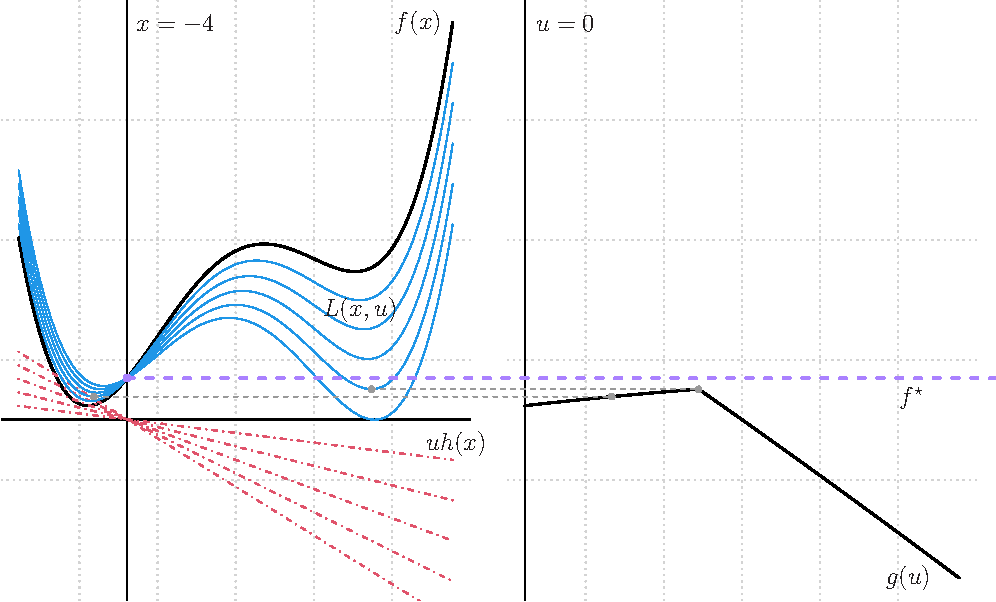
\includegraphics[width=0.89\textwidth]{fig/nonconvex_quartic.pdf}
\caption{Left: the quartic criterion in problem \eqref{eq:nonconvex_quartic},
  drawn as a solid curve. The dashed lines show $uh(x)$ as a function of $x$ for
  different values of the dual variable $u$, where $h(x) = -x-4 \leq 0$ is the
  inequality constraint in \eqref{eq:nonconvex_quartic}. The thin solid curves
  show the Lagrangian $L(x,u)$ as a function of $x$, for the same values of
  $u$. Right: the associated dual function, as in
  \eqref{eq:nonconvex_quartic_dual}, which at each $u$ is given by minimizing 
  $L(x,u)$ over all $x$. The dashed horizontal line marks the optimal primal
  value $f^\star$. We see that weak duality $f^\star \geq g^\star$ holds, and
  the inequality is strict.}   
\label{fig:nonconvex_quartic}
\end{figure}

\section{Interpretations}
\label{sec:duality_interpretations}

In this section, we discuss some interpretations of Lagrange duality. Without
loss of generality, we will simply denote the dual variable by $u$, that is, we
drop reference to the block $v$ corresponding to the equality constraints in the
primal \eqref{eq:primal_problem}. This is possible since equality constraints
can always be rewritten as inequality constraints (each $\ell_j(x) = 0$ can be
rewritten as $\ell_j(x) \leq 0$ and $-\ell_j(x) \leq 0$). 

\paragraph{Max-min interpretation.}
\parlab{par:max_min}

Recall that, by definition \eqref{eq:dual_function}, for each $u \geq 0$,    
\[
\inf_x \, L(x,u) = g(u).
\]
Meanwhile, we also have the following symmetrical fact: for any $x$, 
\[
\sup_{u \geq 0} \, L(x,u) = f(x) + I_C(x),
\]
where $C = \{x : h_i(x) \leq 0, \, i=1,\dots,m\}$ is the primal feasible
set. To see this, note that we have the upper bound $L(x,u) \leq f(x) +
I_C(x)$ for all $x$ and $u \geq 0$. For $x \in C$, the upper bound is attained   
at $u = 0$, whereas for $x \notin C$, the upper bound is attained by sending 
$u_i \to \infty$, where $i$ is such that $h_i(x) > 0$. Therefore by the general
max-min inequality (see Exercise \ref{ex:inf_sup_rules} part d): 
\[
\underbrace{\inf_x \, \sup_{u \geq 0} \, L(x,u)}_{f^\star} \geq 
\underbrace{\sup_{u \geq 0} \, \inf_x \, L(x,u)}_{g^\star}.
\]
This is in fact precisely weak duality \eqref{eq:weak_duality}, since the 
left-hand side is \smash{$f^\star = \inf_x \, \{ f(x) + I_C(x) \}$} and the 
right-hand side is \smash{$g^\star = \sup_{u \geq 0} \, g(u)$}. 

\paragraph{Saddle point interpretation.}

From \eqref{eq:lagrangian_bound1} and \eqref{eq:dual_function}, it follows that  
\[
f(x) \geq L(x,u) \geq g(u), \quad \text{for any primal feasible $x$ and dual
  feasible $u$}, 
\]
where by dual feasible we mean that $u \geq 0$. Suppose that $f^\star =
g^\star$ and $x^\star$ is a solution in the primal problem
\eqref{eq:primal_problem} and $u^\star$ is a solution in the dual problem
\eqref{eq:dual_problem}. Then the inequalities in the last display applied to
$x^\star,u^\star$ must be all equalities:  
\begin{equation}
\label{eq:lagrangian_equalities1}
f(x^\star) = L(x^\star, u^\star) = g(u^\star),
\end{equation}
or equivalently, 
\begin{equation}
\label{eq:lagrangian_equalities2}
\sup_{u \geq 0} \, L(x^\star, u) = L(x^\star, u^\star) = \inf_x \, L(x,
u^\star), 
\end{equation}
where used the definition of $g$ as an infimum, and the supremal representation
of $f$ established in the max-min interpretation, above. Observe that we can
rewrite \eqref{eq:lagrangian_equalities2} as
\index{Lagrangian function!saddle point}
\begin{equation}
\label{eq:lagrangian_saddle_point}
L(x^\star, u) \leq L(x^\star, u^\star) \leq L(x, u^\star), \quad \text{for any
  $x$ and $u \geq 0$},
\end{equation}
which says that $x^\star,u^\star$ is what is known as a \emph{saddle point} of 
the Lagrangian. 

\paragraph{Shadow price interpretation.}

Let us imagine that the primal variable $x$ in \eqref{eq:primal_problem}
represents a planning variable for a given business, and $f(x)$ is the cost 
incurred for operating according to $x$, that is, $-f(x)$ is the profit
earned. Each $h_i(x) \leq 0$ represents an operating constraint, for example, a
space constraint in the current warehouse used by the firm. (Recall, we are
dropping all equality constraints from \eqref{eq:primal_problem}, as we are  
considering the dual variable to be $u \geq 0$.)  Then in this language,
$f^\star$ is the minimal cost (maximum profit) when the firm operates according
to an optimal plan $x^\star$. 

The Lagrangian $L(x,u)$ in this context has the following interpretation. The
business is allowed to break the operating constraints, provided they pay
appropriately for violations. Each component $u_i \geq 0$ of the dual variable
corresponds to a price per unit violation of the constraint $h_i(x) \leq 0$,
that is, $u_i h_i(x)$ represents the cost to the business for violating the
$i\th$ constraint; likewise, $-u_i h_i(x)$ is the profit to the firm for slack
in the $i\th$ constraint. For example, if the firm needs more space, then they
can rent new warehouse space at a price per unit of $u_i$; and if they have
leftover space in their current warehouse, then they can rent it out at the same 
price. The value of the Lagrangian $L(x,u)$ thus represents the total cost
incurred when operating according to $x$, with prices according to $u$. The dual  
variable $u$ is often called the vector of \emph{shadow prices} in this
context. 
\index{Lagrangian function!shadow prices}

Weak duality \eqref{eq:weak_duality} now translates into the the following
statement: the optimal cost $g^\star$ when the firm is allowed to violate
constraints and pay accordingly is at most the optimal cost $f^\star$ when they
must respect the constraints, even at the worst-case prices. Moreover, if indeed
$f^\star = g^\star$, and $u^\star$ is a dual solution, then $u^\star$ represents
a set of prices for which there is no advantage to violating the constraints
versus respecting them.  

\section{Duality gap}

In the above, we discussed interpretations in the case when primal and dual 
optimal values match,       
\index{strong duality}
\begin{equation}
\label{eq:strong_duality}
f^\star = g^\star,
\end{equation}
which is a condition we call \emph{strong duality}. To be clear, unlike weak
duality \eqref{eq:weak_duality}, strong duality is \emph{not} guaranteed to hold
in general, for any given primal problem \eqref{eq:primal_problem} and its dual  
\eqref{eq:dual_problem}. (Recall, the example in Figure
\ref{fig:nonconvex_quartic} demonstrated a failure of strong duality for problem
\eqref{eq:nonconvex_quartic}.) However, it does hold for ``most'' convex
optimization problems, as the next section makes precise. 

A related concept, for primal feasible $x$ and dual feasible $u,v$, is the
quantity  
\index{duality gap}
\begin{equation}
\label{eq:duality_gap}
f(x) - g(u,v) \geq 0,
\end{equation}
which is called the \emph{duality gap} at $x,u,v$. Note that strong duality the
case in which the duality gap is zero at a primal solution $x^\star$ and dual
solution $u^\star, v^\star$ (assuming solutions exist, that is, assuming the
optimal values are achieved).  

Though it is a simple concept, the duality gap is a powerful tool, as the next
result shows.

\begin{Theorem}
\label{thm:duality_gap}
For any primal problem \eqref{eq:primal_problem} and its dual
\eqref{eq:dual_problem}, and any primal feasible $x$ and dual feasible $u,v$,  
the following holds.  

\begin{enumerate}[label=(\roman*)]
\item If the duality gap at $x,u,v$ equals $\epsilon \geq 0$, then $f(x) -
  f^\star \leq \epsilon$, and $g^\star - g(u,v) \leq \epsilon$.  

\item If the duality gap at $x,u,v$ is zero, then $x$ is primal optimal and
  $u,v$ are dual optimal. 
\end{enumerate}
\end{Theorem}

The proof of the theorem is straightforward. If $f(x) - g(u,v) \leq \epsilon$, 
then by virtue of the fact that $f(x) \geq f^\star \geq g^\star \geq g(u,v)$, we
conclude that $f(x) - f^\star \leq \epsilon$ and $g^\star - g(u,v) \leq
\epsilon$, and this proves part (i). Meanwhile, part (ii) simply elucidates the  
special case with $\epsilon = 0$.

This theorem has numerous important implications, both in practice and in 
theory. For example, iterative algorithms which operate on the primal and the
dual simultaneously will be able to use the duality gap as a stopping criterion, 
and in doing so, will stop with a suboptimality guarantee on the primal and the 
dual criteria, by Theorem \ref{thm:duality_gap} part (i).  

As another example, Theorem \ref{thm:duality_gap} part (ii) can be used to
derive a converse of the saddle point property of the last section. There we
proved that if strong duality holds, and $x^\star,u^\star$ are primal and 
solutions, respectively (assuming no equality constraints, without loss of
generality), then $x^\star, u^\star$ is a saddle point of the Lagrangian, as in
\eqref{eq:lagrangian_saddle_point}. Conversely, if the saddle point property 
\eqref{eq:lagrangian_saddle_point} holds at a pair \smash{$\bar{x}, \bar{u}$},
then tracing back to \eqref{eq:lagrangian_equalities2} and
\eqref{eq:lagrangian_equalities1} shows that \smash{$\bar{x}, \bar{u}$} achieve
zero duality gap, which implies they must be optimal. We will revisit the saddle
point perspective in Chapter \ref{sec:saddle_point_condition}.   
\index{Lagrangian function!saddle point}
 
\section{Slater's condition}
\label{sec:slater_condition}

As we have already seen (Example \ref{ex:nonconvex_quartic}), for a nonconvex 
optimization problem, strong duality \eqref{eq:strong_duality} can fail to
hold. Fortunately, strong duality holds for a broad class of convex optimization
problems, as the next theorem makes precise.  

\index{Slater's condition}
\index{strong duality}
\begin{Theorem}
\label{thm:slater_condition}
Consider the optimization problem \eqref{eq:primal_problem}, where after 
relabeling, if needed, we take $h_1, \dots, h_r$ to be inequality constraint
functions which are affine ($r = 0$ if none are affine). Assume the following.         

\begin{enumerate}[label=(\roman*)]
\item The functions $f$ and $h_i$, $i=1,\dots,m$ are convex, and $\ell_j$,
  $j=1,\dots,k$ are affine; in other words, problem \eqref{eq:primal_problem} is
  convex, and we can write its equality constraints as $Ax = b$.      

\item There exists $x \in \relint(D)$, where \smash{$D = \dom(f) \cap
    \bigcap_{i=r+1}^m \dom(h_i)$} denotes the common effective domain, such that      
  \begin{equation}
  \label{eq:slater_condition}
  h_i(x) \leq 0 \;\, \text{for all $i \leq r$}, \quad
  h_i(x) < 0 \;\, \text{for all $i > r$}, \quad Ax = b. 
  \end{equation}
\end{enumerate}

Then strong duality holds: the optimal values $f^\star$ in problem
\eqref{eq:primal_problem} and $g^\star$ in the corresponding dual problem  
\eqref{eq:dual_problem} satisfy $f^\star = g^\star$. 
\end{Theorem}

Taken together, conditions (i) and (ii) in Theorem \ref{thm:slater_condition}
are called \emph{Slater's condition}. In short, this assumes convexity along  
with a type of strict feasibility condition \eqref{eq:slater_condition};
precisely, that there exists a point $x$ (in the relative interior of the domain
$D$) which satisfies the affine equality and inequality constraints and strictly
satisfies the nonaffine inequality constraints. This strict feasibility
condition is very mild, which is why we say that strong duality holds for
``most'' convex problems. The proof of Theorem \ref{thm:slater_condition} is
based on (an intricate application of) the separating hyperplane theorem, and is
outlined in Exercises \ref{ex:convex_theorem_alternatives} and
\ref{ex:slater_condition}.    

We can demonstrate the utility of Slater's condition by revisiting LPs. An LP
\eqref{eq:lp_primal} is always a convex problem, and all of its constraints are
affine, so Slater's condition applied to \eqref{eq:lp_primal} says that strong
duality holds if \eqref{eq:lp_primal} is feasible. Moreover, one can verify
(Exercise \ref{ex:lp_dual_dual}) that the dual of the dual problem
\eqref{eq:lp_dual} is the primal problem \eqref{eq:lp_primal}. Therefore, strong
duality in problems \eqref{eq:lp_primal} and \eqref{eq:lp_dual} refer to the
same thing, and Slater's condition applied to \eqref{eq:lp_dual} shows that
strong duality also holds if \eqref{eq:lp_dual} is feasible. Next, we summarize
these conclusions.  

\index{linear program!strong duality}
\begin{Corollary}
\label{cor:slater_lp}
For an LP, strong duality holds if the primal or the dual problem is 
feasible. 
\end{Corollary}

More can be said, by more precisely characterizing what happens when only one of
the primal or the dual is infeasible; see Exercise \ref{ex:lp_slater}. Exercises
\ref{ex:lasso_dual} and \ref{ex:svm_dual} examine duality in the lasso and SVM
problems (both QPs), and use Slater's condition to conclude that strong duality
always holds.        

\section{SDP duality*}
\label{sec:sdp_duality}

Consider a generic semidefinite program (SDP) of the form
\begin{equation}
\label{eq:sdp_primal}
\begin{alignedat}{2}
&\minimize_x \quad && c^\T x \\
&\st \quad && x_1 A_1 + \cdots + x_d A_d \preceq B \\  
& && Gx = h.
\end{alignedat}
\end{equation}
To construct the Lagrangian dual of \eqref{eq:sdp_primal}, we adopt our standard 
approach of treating the space of symmetric matrices as a vector space with the   
inner product $\langle X, Y \rangle = \tr(XY)$ and partial ordering $X \preceq Y
\iff Y-X \succeq 0$. Just as before, we will associate a dual variable with
each constraint that appears in our primal problem; what this means now is that
we associate a dual matrix $U$ with the inequality constraint
\smash{$\sum_{i=1}^d x_i A_i - B \preceq 0$}, and associate a dual vector $v$
with the equality constraint $Gx - h = 0$. Hence the Lagrangian is   
\[
L(x,U,v) = c^\T x + \bigg\langle U, \sum_{i=1}^d x_i A_i - B \bigg\rangle + v^\T
(Gx - h). 
\]
Now we make use of the following key fact (Exercise
\ref{ex:psd_cone_self_dual}):   
\index{positive semidefinite cone!dual cone}
\begin{equation}
\label{eq:psd_cone_self_dual}
Y \succeq 0 \iff \text{$\tr(XY) \geq 0$ for all $X \succeq 0$}.  
\end{equation}
We will revisit \eqref{eq:psd_cone_self_dual} in Chapter \ref{sec:dual_cones},
where in the language of that chapter, we will learn that it says the positive
semidefinite cone is self-dual. Note that \eqref{eq:psd_cone_self_dual} implies 
for feasible $x$ and $U \succeq 0$,
\[
\bigg\langle U, \sum_{i=1}^d x_i A_i - B \bigg\rangle = \tr \bigg[ U \bigg(
\sum_{i=1}^d x_i A_i - B \bigg) \bigg] \leq 0.
\]
In other words, we see that indeed the Lagrangian satisfies $L(x,U,v) \leq c^\T
x$, for any feasible $x$ and $U,v$ such that $U \succeq 0$, which verifies 
\eqref{eq:lagrangian_bound1} for the current setting. Proceeding as in
\eqref{eq:lagrangian_bound2}, \eqref{eq:dual_function} \eqref{eq:dual_problem},
we minimize the Lagrangian $L(x,U,v)$ over unconstrained $U,v$ to yield the dual
problem:
\index{semidefinite program!dual problem}
\begin{equation}
\label{eq:sdp_dual}
\begin{alignedat}{2}
&\maximize_{U,v} \quad && -\tr(BU) - h^\T v \\
&\st \quad && \tr(A_iU) + g_i^\T v = -c_i, \; i = 1,\dots,d \\
& && U \succeq 0.
\end{alignedat}
\end{equation}
where $g_i$, $i=1,\dots,d$ denote the columns of $G$. Note the close analogy
between \eqref{eq:sdp_dual} and the LP dual \eqref{eq:lp_dual}. For the dual of
an SDP in standard form, see Exercise \ref{ex:sdp_std_dual}. 

By construction, we have that weak duality holds, $f^\star \geq g^\star$,
between \eqref{eq:sdp_primal} and \eqref{eq:sdp_dual}, with $f^\star$ denoting 
the optimal value in \eqref{eq:sdp_primal} and $g^\star$ the optimal value in 
\eqref{eq:sdp_dual}. When does strong duality hold? For this, we need an
extension of Slater's theorem. This will be given later in Chapter
\ref{sec:conic_duality}, when we cover conic duality, and the following is a    
consequence for SDPs. 

\index{semidefinite program!strong duality}
\begin{Corollary}
\label{cor:slater_sdp}
Strong duality holds between the SDP \eqref{eq:sdp_primal} and its dual
\eqref{eq:sdp_dual} in either of the following cases. 

\begin{enumerate}[label=(\roman*)]
\item There exists $x$ such that $Gx = h$ and $x_1 A_1 + \cdots + x_d A_d 
  \prec B$.  
\item There exists $U,v$ such that $\tr(A_iU) + g_i^\T v = -c_i$, $i =
  1,\dots,d$, and $U \succ 0$. 
\end{enumerate}
\end{Corollary}

Like the result for LPs in Corollary \ref{cor:slater_lp}, the result in
Corollary \ref{cor:slater_sdp} is based on the observation that the dual of the 
dual SDP is the primal SDP (Exercise \ref{ex:sdp_dual_dual}), so to obtain
a sufficient condition for strong duality, we can apply Slater's condition to
either the primal SDP and the dual SDP. 

While the theory of duality for SDPs has many similarities to that for LPs, it is
also important to note their differences. For example, the duality gap in an SDP
can be finite and positive, which is impossible in an LP. Exercise
\ref{ex:lp_sdp_differences} explores this and related facts.     

\SkipTocEntry\section*{Chapter notes}

Linear programming was initially the focus in developing the theory of 
duality, as laid out by David Gale, Harold Kuhn, and Albert Tucker in
\cite{gale1951linear}. This grew out of John von Neumman's famous minimax 
theorem in zero-sum, two-player games, published over two decades
earlier in \cite{vonneumann1928theorie} (we return to this and related
saddle point theorems in Chapter \ref{sec:minimax_theorems}). Historical
notes, tracing through the contributions of these and other authors, can be
found in the commentary section in Chapter 11 of
\cite{rockafellar2009variational}, among other places.

Duality is given an in depth treatment in many standard references, such as
\cite{rockafellar1970convex} (Chapters 27--32), \cite{boyd2004convex} (Chapter  
5), and \cite{bertsekas2009convex} (Chapters 4, 5). These books take on
somewhat different perspectives: Rockafellar builds up duality via conjugacy
operations, Bertsekas pursues a geometric theory based on min common/max
crossing duality, whereas Boyd and Vandenberghe take a more Lagrangian-centric 
view, and present numerous interpretations and examples of dual problems. Our
presentation is inspired in large part by \cite{boyd2004convex}. What we call
Slater's condition, in Theorem \ref{thm:slater_condition}, is called
\emph{relaxed} Slater's condition by Boyd and Vandenberghe and other
authors. Slater's condition is named after \cite{slater1950lagrange}.  

The lecture notes of \cite{bental2023convex} (Chapter 3) are a rich, advanced
resource on duality. Working in a vector space endowed with conic ordering,
these authors develop a convex theorem of alternatives, dual problems, and
optimality conditions---all from first principles. Our treatment of conic 
duality, in Chapter \ref{sec:conic_duality}, is based on theirs. A consequence
of this more general conic duality theory is the strong duality result for SDPs
in Corollary \ref{cor:slater_sdp}. Exercises
\ref{ex:convex_theorem_alternatives} and \ref{ex:slater_condition} are based on
\cite{bental2023convex}.            
 
\clearpage

\begin{xcb}{Exercises}
\begin{enumerate}[label=\thechapter.\arabic*]
\settowidth{\leftmargini}{0.00.\hskip\labelsep}
\index{linear program!dual problem}
\index{linear program!standard form}
\item \label{ex:lp_std_dual}
  Consider the standard form LP,
  \begin{alignat*}{2}
  &\minimize_x \quad && c^\T x \\
  &\st \quad && Ax = b \\
  & && x \geq 0.
  \end{alignat*}
  Prove that its dual problem is 
%  \label{eq:lp_std_dual}
  \begin{alignat*}{2}
  &\maximize_{u,v} \quad && b^\T v \\
  &\st \quad && A^\T v + u = c \\
  & && u \geq 0.
  \end{alignat*}

\index{quadratic program!dual problem}
\index{quadratic program!standard form}
\item \label{ex:qp_std_dual} 
  Consider the standard form QP,
  \begin{alignat*}{2}
  &\minimize_x \quad && \frac{1}{2} x^\T Q x + c^\T x \\
  &\st \quad && Ax = b \\
  & && x \geq 0,
  \end{alignat*}
  with $Q \succ 0$. Prove that its dual problem is
%  \label{eq:lp_std_dual}
  \begin{alignat*}{2}
  &\maximize_{u,v} \quad && -\frac{1}{2} (c - A^\T v - u)^\T Q^{-1} (c - A^\T v
  - u) + b^\T v \\
  &\st \quad && A^\T v + u = c \\
  & && u \geq 0.
  \end{alignat*}

\index{quadratic program!dual problem}
\item \label{ex:qp_psd_dual} 
  Consider the QP in \eqref{eq:qp_primal} but now assume that $Q \succeq
  0$. Prove that its dual is as claimed in \eqref{eq:qp_psd_dual}. Hint: take
  the gradient of the Lagrangian with respect to $x$, then set it equal to zero
  and rearrange to yield $Qx = -(c + A^\T u + G^\T v)$. When does this have a  
  solution? When this does not have a solution, what does that mean about the 
  infimum of the Lagrangian over $x$?   

\item \label{ex:nonconvex_quartic}
  We derive the dual for the nonconvex quartic minimization
  \eqref{eq:nonconvex_quartic}, as claimed in Example
  \ref{xa:nonconvex_quartic}. First show that taking the derivative of the
  Lagrangian with respect to $x$ and setting it equal to zero leads to
  \[
  x^3 - 25x + 25 - \frac{25}{2} u = 0.
  \]
  This is called a \emph{depressed} cubic equation, since it does not have any 
  term involving $x^2$. Show that Cardano's formula, for the roots of a
  depressed cubic, yields the three roots $x = R_j(u)$, $j = 1,2,3,\dots$ as
  defined in the example. Then argue that the dual function $g$ in 
  \eqref{eq:nonconvex_quartic_dual} can be obtained by taking the minimum value
  of the (real part of the) Lagrangian over these roots. 

\item The transportation problem from Example \parref{xa:transportation}   
  offers an intuitive example of LP duality. In this setting, recall, we have a
  per unit transportation cost $c_{ij}$ from location $i$ to $j$, a supply $s_i$
  at $i$, and a demand $d_j$ at $j$. The problem is to minimize the total
  transportation cost:  
  \begin{alignat*}{2}
  &\minimize_x \quad && \sum_{i=1}^m \sum_{j=1}^n c_{ij} x_{ij} \\ 
  &\st \quad && \sum_{j=1}^n x_{ij} = s_i, \; i=1,\dots,m \\
  & && \sum_{i=1}^m x_{ij} = d_j, \; j=1,\dots,n \\
  & && x \geq 0.
  \end{alignat*}
  Prove that its dual is (equivalent to, after reparametrization):    
  \begin{alignat*}{2}
  &\maximize_{u,v} \quad && \sum_{i=1}^m u_i s_i + \sum_{j=1}^n v_j d_j \\  
  &\st \quad && u_i + v_i \leq c_{ij}, \; i=1,\dots,m, \; j=1,\dots,n,
  \end{alignat*}
  which is sometimes referred to as the \emph{shipper's problem}. The
  interpretation is as follows. A shipper puts forth a proposal to charge $u_i$
  to load each unit from location $i$ and $v_j$ to unload each unit from
  location $j$. The shipper will try to maximize their profit, but must not
  charge more to ship from $i$ to $j$ than the given cost $c_{ij}$. By strong
  duality, a clever shipper (with dual optimal prices) will make exactly as much
  as the cheapest possible transportation cost.    
 
\item \label{ex:lp_dual_dual}
  To form the dual of \eqref{eq:lp_dual}, first convert it to a minimization
  problem by negating its criterion and rewrite the equality constraint as
  $-A^\T u - G^\T v = c$. Then simply pursue the usual steps in Lagrangian
  duality, as in Chapter \ref{sec:lagrangian_duality}. Show that this gives       
  \begin{alignat*}{2}
  &\maximize_{x,y} \quad && -c^\T x \\ 
  &\st \quad &&  Ax + y = b \\
  & && Gx = h \\
  & && y \geq 0.
  \end{alignat*}
  After eliminating $y$ and negating the criterion to convert this to a
  minimization problem, show that we arrive back at \eqref{eq:lp_primal}.  

\index{linear program!strong duality}
\item \label{ex:lp_slater}
  Prove the following refinement of Corollary \ref{cor:slater_lp} for LPs. We
  use $f^\star, g^\star$ for the optimal values in \eqref{eq:lp_primal},
  \eqref{eq:lp_dual} respectively. 

\begin{enumerate}[label=\alph*.]
\item If both the primal \eqref{eq:lp_primal} and dual \eqref{eq:lp_dual} are
  infeasible, then strong duality fails.

\item If either the primal \eqref{eq:lp_primal} or dual \eqref{eq:lp_dual} are
  feasible, then strong duality holds.

\item If the primal \eqref{eq:lp_primal} is feasible, then $f^\star > -\infty$ 
  if and only if the dual \eqref{eq:lp_dual} is feasible.   

\item If the dual \eqref{eq:lp_dual} is feasible, then $g^\star < \infty$ if and
  only if the primal \eqref{eq:lp_primal} is feasible.     
\end{enumerate}

\item \label{ex:lasso_dual}
  Consider the lasso problem, for a response vector $y \in \R^n$ and feature   
  matrix $X \in \R^{n \times d}$, 
  \[
  \minimize_\beta \quad \frac{1}{2} \|y - X \beta\|_2^2 + \lambda \|\beta\|_1. 
  \]
  To apply Lagrangian duality, we introduce an auxiliary variable, rewriting
  this as     
  \begin{equation}
  \label{eq:lasso_primal}
  \minimize_{\beta,z} \quad \frac{1}{2} \|y - z\|_2^2 + \lambda \|\beta\|_1  
  \quad \st \quad z = X \beta.
  \end{equation}

\begin{enumerate}[label=\alph*.]
\item Show that the dual of \eqref{eq:lasso_primal} is (equivalent to)
  \index{lasso!dual problem} 
  \begin{equation}
  \label{eq:lasso_dual}
  \maximize_u \quad -\frac{1}{2} \|y - u\|_2^2 + \frac{1}{2} \|y\|_2^2 \quad \st
  \quad \|X^\T u\|_\infty \leq \lambda.
  \end{equation}

\item Use Slater's condition to show that strong duality always holds between 
  \eqref{eq:lasso_primal}, \eqref{eq:lasso_dual}.  
\end{enumerate}

\item \label{ex:svm_dual}
  Consider the SVM problem, for labels $y_i \in \{ -1, 1\}$ and features $x_i
  \in \R^d$, $i=1,\dots,n$,       
  \begin{equation}
  \label{eq:svm_primal}
  \begin{alignedat}{2}
  &\minimize_{\beta_0,\beta,\xi} \quad
  && \frac{1}{2} \|\beta\|_2^2 + C \sum_{i=1}^n \xi_i \\ 
  &\st \quad && y_i (\beta_0 + x_i^\T \beta) \geq 1-\xi_i, \;  i=1,\dots,n \\ 
  & && \xi \geq 0.
  \end{alignedat}
  \end{equation}

\begin{enumerate}[label=\alph*.]
\item Let $y \in \R^n$ denote the label vector and $X \in \R^{n \times d}$ the
  feature matrix (whose $i\th$ row is $x_i^\T$), and define \smash{$\tilde{X} =
    \diag(y) X$}. Show that the dual of \eqref{eq:svm_primal} is (equivalent to)      
  \index{support vector machine!dual problem} 
  \begin{equation}
  \label{eq:svm_dual}
  \begin{alignedat}{2}
  &\maximize_\alpha \quad &&-\frac{1}{2} \alpha^\T \tilde{X} \tilde{X}^\T \alpha
  + \one^\T \alpha \\    
  &\st \quad && 0 \leq \alpha \leq C \one \\
  & && y^\T \alpha = 0.
  \end{alignedat}
  \end{equation}

\item Use Slater's condition to show that strong duality always holds between   
  \eqref{eq:svm_primal}, \eqref{eq:svm_dual}.  
\end{enumerate}

\index{Farkas' lemma}
\item \label{ex:farkas_variations}
  We will examine a couple of variations on Farkas' lemma, the second of which 
  will be critical for proving the convex theorem of alternatives in the next
  exercise.      

\begin{enumerate}[label=\alph*.]
\item Given $A \in \R^{k \times d}$ and $b \in \R^k$, consider two statements: 
  \begin{itemize}
  \item for all $x \in \R^d$, it holds that $Ax \leq 0 \implies a^\T x \leq 0$;  
  \item there exists $\mu \in \R^k$ such that $\mu \geq 0$ and $A^\T \mu = 
    a$.
  \end{itemize}
  Prove that these are equivalent statements. Hint: showing that the second  
  implies the first is straightforward. To prove the other direction, apply
  Farkas' lemma, Exercise \ref{ex:farkas_lemma}, with $A,b$ replaced by $-A^\T,
  -a$, respectively.        

\item Given $A \in \R^{k \times d}$, $b \in \R^k$, $g \in \R^d$, and $h \in \R$,
  where $b \geq 0$, consider two statements:  
  \begin{itemize}
  \item for all $x \in \R^d$, it holds that $Ax \leq b \implies g^\T x \leq h$;  
  \item there exists $\mu \in \R^k$ such that $\mu \geq 0$ and $\mu^\T (Ax - b) 
    \geq g^\T x - h$ for all $x \in \R^d$.
  \end{itemize}
  Prove that these are equivalent statements. Hint: as before, showing the
  second implies the first is straightforward. For the other direction, start by
  defining 
  \[
  C = \bigg\{ \begin{bmatrix} A \\ -g^\T \end{bmatrix} x + \begin{bmatrix} u \\     
    v \end{bmatrix} : x \in \R^d, \, u \in \R^k_+, \, v > 0 \bigg\} 
  \quad \text{and} \quad D = \bigg\{ \begin{bmatrix} b \\ -h \end{bmatrix} 
  \bigg\},
  \] 
  and apply the separating hyperplane theorem, Theorem
  \ref{thm:separating_hyperplane}, to show that there exists a nonzero vector
  $(s,t) \in \R^d \times \R$ such that 
  \[
  s^\T (Ax - b) \geq t (g^\T x - h), \quad \text{for all $x \in \R^d$}.
  \]
  Argue that $A^\T s = ts$, $s \geq 0$, and $t \geq 0$; otherwise the claimed
  separation is not possible. Further, argue that $\tau > 0$; otherwise it
  follows that $A^\T s = 0$ and $b^\T s = 0$, which---after reparametrizing the  
  original space from $\R^k$ to $\col([A \; b])$, if needed---implies that $s = 
  0$. Thus, with $t > 0$, define $\mu = s/t$ in order to prove the desired
  conclusion.           
\end{enumerate}

\item \label{ex:convex_theorem_alternatives}
  Given functions $f$, $h_i$, $i=1,\dots,m$, and $\ell_j$, $j=1,\dots,k$,
  consider the feasibility problems:
  \begin{align}
  \label{eq:feasibility_problem1}
  &\begin{alignedat}{2}  
  &\find \quad && x \\ 
  &\st \quad && f(x) < c \\
  & && h_i(x) \leq 0, \; i = 1,\dots,m \\
  & && \ell_j(x) = 0, \; j = 1,\dots,k,
  \end{alignedat} \\[10pt]
  \label{eq:feasibility_problem2}
  &\begin{alignedat}{2}  
  &\find \quad && u,v \\ 
  &\st \quad && \inf_x \, \bigg\{ f(x) + \sum_{i=1}^m u_i h_i(x) + \sum_{j=1}^k 
  v_j \ell_j(x) \bigg\} \geq c \\
  & && u \geq 0.
  \end{alignedat}
  \end{align}
  The value of $c$ here is fixed and arbitrary. Following Theorem
  3.2.1 in \cite{bental2023convex}, we will prove what these authors call the 
  \emph{convex theorem of alternatives}, which says that under conditions (i)
  and (ii) in Theorem \ref{thm:slater_condition}, problem
  \eqref{eq:feasibility_problem2} is feasible if and only if
  \eqref{eq:feasibility_problem1} is infeasible.            
  
\begin{enumerate}[label=\alph*.]
\item Assume that problem \eqref{eq:feasibility_problem2} is feasible. Prove
  that \eqref{eq:feasibility_problem1} is infeasible. Hint: argue the
  contrapositive. Note that this part of the argument does not use Slater's
  condition.          
  
\item The other direction---that infeasibility of problem
  \eqref{eq:feasibility_problem1} implies feasibility of
  \eqref{eq:feasibility_problem2}---is considerably more involved, and we will
  prove this in several steps. To simplify notation, we will assume without a
  loss of generality that $c = 0$, and that $x = 0$ satisfies condition (ii) in
  Theorem \ref{thm:slater_condition}. Moreover, for the remainder of this proof,
  we will:    
  \begin{itemize}  
  \item redefine $A,b$ such that $Ax \leq b$ represents the affine inequality 
    constraints in \eqref{eq:feasibility_problem1} (originally represented as 
    $h_1(x) \leq 0, \dots, h_r(x) \leq 0$, and $\ell_1(x) = 0, \dots, \ell_k(x)
    = 0$), then relabel the corresponding dual variable as $v \geq 0$;     
  \item redefine $h$ such that $h_1(x) \leq 0, \dots, h_m(x) \leq 0$ represents 
    the nonaffine inequality constraints in \eqref{eq:feasibility_problem1}
    (originally represented as $h_{r+1}(x) \leq 0, \dots, h_m(x) \leq 0$), then
    relabel the corresponding dual variable as $u \geq 0$.  
  \end{itemize}
  We will maintain $m,k$ for the dimensions of $u,v$, respectively. Now define
  the sets     
  \begin{align*}
  S &= \Big\{ (t_0, t_1) \in \R \times \R^m : t_0 < 0, \, t_1 \leq 0 \Big\}, \\  
  T &= \Big\{ (t_0, t_1) \in \R \times \R^m : \text{there exists $x$ such that
      $f(x) \leq t_0$, $h(x) \leq t_1$, and $Ax \leq b$} \Big\}. 
  \end{align*}
  Assume that \eqref{eq:feasibility_problem1} is infeasible. Prove that there
  exists a nonzero vector $a = (a_0, a_1) \in \R \times \R^m$, with $a \geq 0$,
  such that  
  \[
  \inf_{t \in T} \, a^\T t \geq 0.  
  \]
  Hint: apply the separating hyperplane theorem, Theorem
  \ref{thm:separating_hyperplane}, to $S,T$. Then argue that we must have $a
  \geq 0$ and $b = 0$ in the definition of the supporting hyperplane. 

\item Prove that $a_0 > 0$. Hint: assume in order to achieve a contradiction 
  that $a_0 = 0$. Then use $(f(0), h(0)) \in T$, and the fact that $x = 0$
  satisfies condition (ii) in Theorem \ref{thm:slater_condition}, by assumption,
  to conclude $a_1 = 0$.
\item Define $\alpha = a_1 / a_0 \in \R^m$, and  
  \[
  F(x) = f(x) + \alpha^\T h(x),
  \]
  where $h(x) = (h_1(x), \dots, h_m(x))$. Noting that $\alpha \geq 0$ (since
  $a_0 > 0$ and $a_1 \geq 0$), prove
  \[
 \text{for all $x$}, \quad Ax \leq b \implies F(x) \geq 0.
  \]
  Hint: for any $Ax \leq b$, we have $t = (f(x), h(x)) \in T$, so that $a^\T t
  \geq 0$.

\item In what remains, we seek to show that there exists $\beta \in \R^k$ such
  that $\beta \geq 0$ and  
  \begin{equation}
  \label{eq:feasibility_problem3}
  F(x) + \beta^\T (Ax - b) \geq 0, \quad \text{for all $x$}. 
  \end{equation}
  Notice that this would complete the proof as it would verify that 
  \eqref{eq:feasibility_problem2} is feasible, with $u = \alpha$ and $v = \beta$ 
  (recall that we have relabeled the constraint system and taken $c =
  0$). Towards verifying the existence of such a vector $\beta$, define the sets   
  \begin{align*}
  G &= \Big\{ (x, z) \in \R^d \times \R : Ax \leq b, \, z < 0 \Big\}, \\   
  H &= \Big\{ (x, z) \in \R^d \times \R : F(x) \leq z \Big\}. 
  \end{align*}
  Prove that there exists a nonzero vector $(w, \eta) \in \R^d \times \R$ such
  that  
  \[
  \sup \, \Big\{ w^\T x + \eta z : Ax \leq b, \, z < 0 \Big\} \leq \inf \,
  \Big\{ w^\T x + \eta z : F(x) \leq z \Big\}.  
  \]
  Hint: apply the separating hyperplane theorem again, this time to $G,H$.

\item Argue that $\eta \geq 0$, so that 
  \[
  \sup \, \Big\{ w^\T x : Ax \leq b \Big\} \leq \inf \, \Big\{ w^\T x + \eta
  F(x) : x \in \R^d \Big\}.
  \]

\item Argue further that $\eta > 0$, so that by defining $\rho = w / z$, we 
  have  
  \[
  \sup \, \Big\{ \rho^\T x : Ax \leq b \Big\} \leq \inf \, \Big\{ \rho^\T x +
  F(x) : x \in \R^d \Big\}. 
  \]
  Hint: assume for the sake of contradiction that $\eta = 0$. Then as the
  origin $x = 0$ satisfies $Ax \leq b$ (by assumption), the left-hand side in
  the display from part f is at least zero, so that $w^\T x \geq 0$ for all $x$, 
  which can only happen if $w = 0$.     

\item Let $\theta = \sup \, \{\rho^\T x : Ax \leq b\}$. Then $Ax \leq b
  \implies \rho^\T x \leq \theta$, hence by Exercise \ref{ex:farkas_variations} 
  part b, there exists a vector $\beta \geq 0$ such that $\beta^\T (Ax - b) \geq 
  \rho^\T x - \theta$ for all $x$. Use this along with part g to establish
  \eqref{eq:feasibility_problem3} and complete the proof. 
\end{enumerate}

\index{Slater's condition}
\item \label{ex:slater_condition}
  In this exercise, we prove Slater's condition for strong duality, in Theorem 
  \ref{thm:slater_condition}. Let $f^\star, g^\star$ be the optimal values in 
  \eqref{eq:primal_problem} and \eqref{eq:dual_problem}, respectively. Notice
  that if $f^\star = -\infty$, then the desired conclusion $f^\star = g^\star$
  is already implied by weak duality. Hence, assume that $f^\star >
  -\infty$, and use the result in Exercise \ref{ex:convex_theorem_alternatives}
  to prove $f^\star = g^\star$. Hint: set $c = f^\star$.  

\index{positive semidefinite cone!dual cone}
\item \label{ex:psd_cone_self_dual}
  We will prove \eqref{eq:psd_cone_self_dual}. 

\begin{enumerate}[label=\alph*.]
\item If $\tr(XY) \geq 0$ for all $X \in \SS_+^d$, then show that $Y \in
  \SS_+^d$. Hint: consider $X = a a^\T$ for an arbitrary vector $a \in \R^d$.  

\item If $Y \in \SS_+^d$, then show $\tr(XY) \geq 0$ for all $X \in
  \SS_+^d$. Hint: for $X \in \SS_+^d$, prove that we can always write \smash{$X
    = \sum_{i=1}^d x_i x_i^\T$} for vectors $x_i \in \R^d$, $i = 1,\dots,d$. 
\end{enumerate}

\index{semidefinite program!dual problem}
\index{semidefinite program!standard form}
\item \label{ex:sdp_std_dual} 
  Consider the standard form SDP,
  \begin{alignat*}{2}
  &\minimize_X \quad && \langle C, X \rangle \\
  &\st \quad && \langle A_i, X \rangle = b_i, \; i=1,\dots,m \\
  & && X \succeq 0.
  \end{alignat*}
  Prove that its dual problem is 
  \begin{alignat*}{2}
  &\maximize_{U,v} \quad && b^\T v \\
  &\st \quad && v_1 A_1 + \cdots v_m A_m + U = C \\
  & && U \succeq 0.
  \end{alignat*}

\item \label{ex:sdp_dual_dual}
  To form the dual of \eqref{eq:sdp_dual}, first convert it to a minimization
  problem by negating its criterion and rewrite the equality constraints as
  $-\tr(A_iU) - g_i^\T v = c_i$, $i = 1,\dots,d$. Then simply follow the usual
  steps in SDP (Lagrangian) duality, as in Chapter \ref{sec:sdp_duality}. Show
  that this gives    
  \begin{alignat*}{2}
  &\maximize_{x,Y} \quad && -c^\T x \\ 
  &\st \quad && x_1 A_1 + \cdots + x_d A_d + Y = B \\
  & && Gx = h \\
  & && Y \succeq 0.
  \end{alignat*}
  After eliminating $Y$ and negating the criterion to convert this to a
  minimization problem, show that we arrive back at \eqref{eq:sdp_primal}.  

\item \label{ex:lp_sdp_differences}
  LPs and SDPs have several notable differences. First, we can note a difference
  in existence of solutions:
  \begin{itemize}
  \item for an LP, a solution exists whenever its optimal criterion value is
    finite (Corollary \ref{cor:weierstrass_convex_constrained}, which applies
    because for a finite optimal value, the criterion and constraint set cannot
    share a ``proper'' direction of recession along which the criterion is
    nonconstant and the constraint set nonlinear);     
  \item for an SDP, a solution can fail to exist even if the optimal value is
    finite (Exercise \ref{ex:sdp_no_solution}).   
  \end{itemize}
  Moreover, there are notable differences in duality-based perspectives for
  existence of solutions and duality theory more broadly, as we explore in the
  parts below. 

\begin{enumerate}[label=\alph*.]
\item For an SDP \eqref{eq:sdp_primal} which satisfies condition (i) in
  Corollary \ref{cor:slater_sdp}, prove that $f^\star > -\infty$ if and only if
  the dual \eqref{eq:sdp_primal} is feasible, in which case a dual solution
  exists. Hint: apply the general Slater condition from Theorem
  \ref{thm:slater_conic}.    

\item Relatedly, for an SDP whose dual \eqref{eq:sdp_dual} satisfies condition
  (ii) in Corollary \ref{cor:slater_sdp}, prove that $g^\star < \infty$ if and
  only if the primal \eqref{eq:sdp_primal} is feasible, in which case a primal
  solution exists. Hint: apply the general Slater condition from Theorem
  \ref{thm:slater_conic}, now on the dual.  

\item The above results for SDPs can be compared to what is known for LPs, in
  Exercise \ref{ex:lp_slater} parts c and d, where the conclusion is that a
  finite optimal criterion value implies \emph{both} primal and dual LP 
  solutions exist. Show that the statements above, in parts a and b of this
  exercise, cannot be sharpened in general for SDPs by studying the example        
  \begin{alignat*}{2}
   &\minimize_x \quad && x_1 \\
   &\st \quad && 
   \begin{bmatrix}
   x_1 & 1 \\
   1 & x_2 
 \end{bmatrix} \succeq 0.  
  \end{alignat*}
  Show that the primal optimal value is unattained (primal solution does not
  exist), but the dual optimal value is attained (dual solution exists), and
  equals the primal optimal value. Explain why this example does not violate
  parts a and b above. 

\item Show that for an LP, the duality gap $f^\star - g^\star$ can only ever be
  $0$ or $+\infty$. Hint: parts a and b of Exercise \ref{ex:lp_slater}. 

\item Show that for an SDP, the duality gap $f^\star - g^\star$ can be positive
  and finite, by studying the example 
  \begin{alignat*}{2}
   &\minimize_x \quad && x_2 \\
   &\st \quad && 
   \begin{bmatrix}
   x_2 & 0 & 0 \\
   0 & x_1 & x_2 \\
   0 & x_2 & 0 
 \end{bmatrix} \preceq  
 \begin{bmatrix}
  \alpha & 0 & 0 \\
  0 & 0 & 0 \\
  0 & 0 & 0 
 \end{bmatrix}.
  \end{alignat*}
  for arbitrary $\alpha > 0$. Compute the primal optimal value, then compute the
  dual optimal value, to conclude that the duality gap is $\alpha$. Explain why 
  this example does not violate Theorem \ref{thm:slater_conic}. Note: this
  example is taken from \cite{ramana1997exact}, who in turn credits
  \cite{vandenberghe1996semidefinite} for a related example.  
\end{enumerate}

\index{trace norm}
\index{semidefinite program!dual program}
\item \label{ex:trace_norm_semidefinite} 
  This exercise investigates relationships involving the trace norm
  $\|X\|_{\tr}$ of a matrix $X \in \R^{d \times k}$, using SDP duality. 

\begin{enumerate}[label=\alph*.]
\item Show that the $\|X\|_{\tr}$ is the optimal value of the following convex
  optimization (concave maximization) problem:
  \begin{alignat*}{2}
  &\maximize_Y \quad && \tr(X^T Y) \\
  &\st \quad && \begin{bmatrix} I & Y \\ 
    Y^T & I \end{bmatrix} \succeq 0.
  \end{alignat*}
  Hint: use properties of Schur complements, as reviewed in Appendix
  \ref{sec:schur_complement}.

\item Show that the dual associated with the problem in part a is 
  \begin{alignat*}{2}
  &\minimize_{U,V} \quad && \tr(U) + \tr(V) \\
  &\st \quad && \begin{bmatrix} U & \frac{1}{2} X^\T \\  
    \frac{1}{2} X & V \end{bmatrix} \succeq 0.
  \end{alignat*}

\item Show that the optimal values for the problems in parts a and b are equal
  to each other, and both are attained. Hint: for attainment, use Theorem
  \ref{thm:slater_conic}.   

\item Confirm that the two problems in Property
  \parref{par:trace_norm_semidefinite} are equivalent, as claimed.
\end{enumerate}
\end{enumerate}
\end{xcb}
